\chapter{Methodology}
\label{chap:methodology}

[Describes the approach and techniques employed to address the problem. This could include research methods, tools, technologies, and frameworks used during the project and the 3rd semester courses.

You build the project based on the experience and knowledge accumulated during the previous semesters---don't forget that.]

\begin{figure}[htbp]
    \centering
    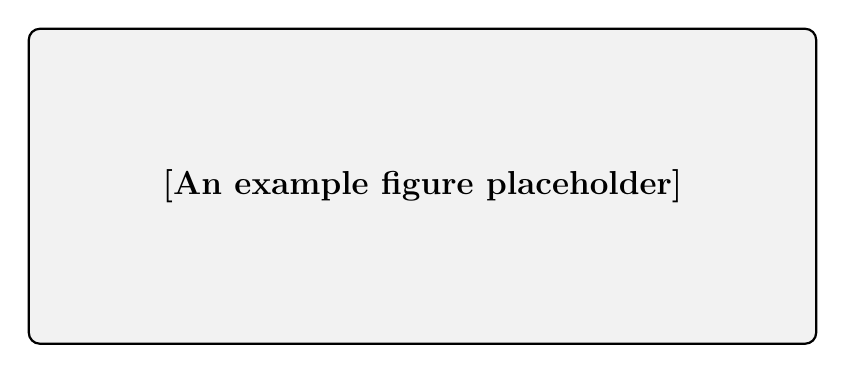
\begin{tikzpicture}
        \draw[thick, fill=gray!10, rounded corners=4pt] (0,0) rectangle (10, 4);
        \node at (5, 2) {\large \textbf{[An example figure placeholder]}};
    \end{tikzpicture}
    \caption{An example figure}
    \label{fig:example_figure}
\end{figure}

\section{[Sub-section]}
\label{sec:methodology_subsection}
[Lorem ipsum]

\subsection{[Sub-sub-section]}
\label{subsec:methodology_subsubsection}
[Lorem ipsum]

